\chapter{Experimental Setup}
In the following sections the experimental setup for this thesis - the Belle II detector and the SuperKEKB collider - are described as far as it is necessary for the tracking software. Detailed information can be found elsewhere \cite{tdr}.


\section{SuperKEKB and the Belle II Detector}

The future Belle II is currently being build at the KEK high energy research facility in Tsukuba, Japan. It is a general purpose $4\pi$ detector for high energy particle experiments. A scheme of the whole detector with the planned measuring devices can be found in figure \ref{fig-belle2}.

The Belle II detector is used for measuring the electron positron collisions induced by the SuperKEKB collider. As its predecessor KEKB its center of mass energy is tuned in such a way that it lays near the $\PgUc$ resonance. This beam energy is chosen that way because a $\PgUc$ particle decays in nearly all cases into a pair of B-mesons. The daughter particles of these B mesons open a window to a very wide window of physical studies like CP violation or B-meson spectroscopy. The energy of the colliding electrons an positrons is asymmetric which leads to a slightly asymmetric collision as well. This fact is exploited in measuring the decay length of the two formed B-Mesons - one of the main ingredients for quantifying the CP violation in the B-Meson system. The usage of electrons and their antiparticles for collisions leads to very clean events compared to other collision partners like protons or even gold atoms. Clean means in this context a reduced number of created decay products (only 11 charged tracks on average) and more or less no pile up (only one collision occurring at the same time) are expected. These circumstances can be used for high precision measurements on the formed particles.

\begin{figure}
 \centering
 \includegraphics[width=0.8\linewidth]{figures/experimental_setup/detector_crossection_labels.pdf}
 \caption{Scheme showing the planned Belle II detector in top view. The single measuring devices are shown with their names. Some more information on the tracking devices can be found in the text. Taken from \cite{christian}.}
 \label{fig-belle2}
\end{figure}

\section{The Tracking Detectors}

As every general purpose high energy particle physics detector the Belle II detector is composed of several single measuring devices - each one with a different task. For collecting as many information on the physical process in the collision as many infromation on the created decay products are needed. These include
\begin{zlist}
 \item Identification of the created particles (for example by their mass),
 \item Measurement of the kinematic properties (like momentum and energy) of the charged particles,
 \item Resolution of their origin position - also called their vertex.
\end{zlist}

The tracking detectors described in this thesis are mainly for recording the momenta of the particles as well as their vertex position. Further more special applications are identification of the particle type by their energy loss.

The measuring principle of the momentum and also the vertex is to let the charge particles fly throw a sensor region with space-resolved measurement and obtain their full path through the detector - a so called track - by combining the different location information - the so called hits. By applying a magnetic field - in Belle II it has a nominal field strength of $B = \unit[1.5]{T}$ parallel to the beam axis - the $z$ axis in the coordinate system of the detector - the charged particle are curled. By measuring the curvature of the curled tracks an estimation of the momentum in the plane perpendicular to the beam axis - the $r$-$\phi$-plane - can be made. The remaining $z$-direction parallel to the beam axis can be computed with the angle of the track to the beam axis.

There exist many different ways to measure the position of a charge particle. Each of them exploits the charge of the particles and their interaction with materials which makes these techniques unusable for neutral particles. In the following two of the used ways in Belle II are described in more detail.

\subsection{CDC}

CDC is an acronym for Central Drift Chamber and is the largest tracking detector in Belle 2. The CDC is a typical gas chamber detector with 14336 sense wires arranged in 56 layer and 9 superlayers. These wires are strained mostly parallel to the beam axis in a cylindrical tank flooded with gas. The gas is a mixture of 50 \% helium and 50 \% ethane. For more information on gas chamber detectors see for example \cite{grupen}.
Each charged particle produced in the collision of the electron and position interacts with the gas and can ionize the helium atoms. The energy deposit of a charged particle is given by the Bethe formula \cite{bethe}
\begin{align}
 - \left\langle \dd{E}{x} \right\rangle = \frac{4 \pi n z^2}{m_e c^2 \beta^2} \cdot \left( \frac{e^2}{4 \pi \varepsilon_0} \right)^2 \left[ \ln\left( \frac{2 m_e c^2 \beta^2}{I(1 - \beta^2} \right) - \beta^2 \right]
\end{align}
which describes the average energy per travel length. This energy is transfered to the shell electrons of the helium gas atoms. As the ionization energy of helium is very low (about $\unit[20]{eV}$) compared to the typical particle energies (up to several $\unit[100]{eV}$) the helium atoms release their electrons very easily. These free electrons get accelerated in the electric field induced between the sense wires and field wires with a high negative voltage attached. An instructive simulation of the typical electronic field distribution between 7 sense wires and 34 field wires can be found in figure \ref{fig-sense-wires}. As the electric field near the sense wires increases with $\propto 1/r$ the free electrons gain more and more energy so that they can ionize helium atoms by themselves as well. This whole flood of free charge can be detected by the electronics attaches to the sense wires and produce a sharp peak there. The more immobile helium atomic cores get absorbed later by the field wires. Because the free electrons have to drift through the gas the measured peak has a delay up to $\unit[500]{ns}$ for the largest drift cells to the initial charged particle passage. With analysis the time and location information of each measured peak the path of the charged particle through the CDC can be reconstructed. A typical event display of the simulated passage of one charge pion with $\unit[1]{GeV}$ can be seen in figure \ref{fig-event-display}. Each wire and each drift cell is almost rotationally symmetric. Therefore there is no way in obtaining information on the direction of the electron flood hitting the sense wire. Therefore each hit produced a so called drift circle rather than a single hit point. These drift circled can also be seen in the figure.

If all CDC wires were strained parallel to the beam axis there were no way in measuring the angle between the charged particles and the beam axis. That is the reason why some of the wires are installed with a small tilting angle. These wires are called stereo wires in contrast to the axial wires without tilting angle. A measured hit on the stereo wires does not give information neither on the position along the beam axis nor in the layer parallel to it. Only the information collected among all axial and stereo hits lead to a correct estimation of the momentum in all directions. A sketch of some axial and stereo wires sharing the same distance from the beam axis - also called a layer of wires - are shown in \ref{fig-axial-stereo}.

\begin{SCfigure}
  \caption{Simulation of the electron field in an extract of the wires in the central drift chamber. The violet circles depict the field wires whereas the red small points are the sense wires. The yellow paths are examples for the drift paths of ionized electrons. This simulation includes the distortion by the magnetic field. Taken from \cite{cdc_design}.}
  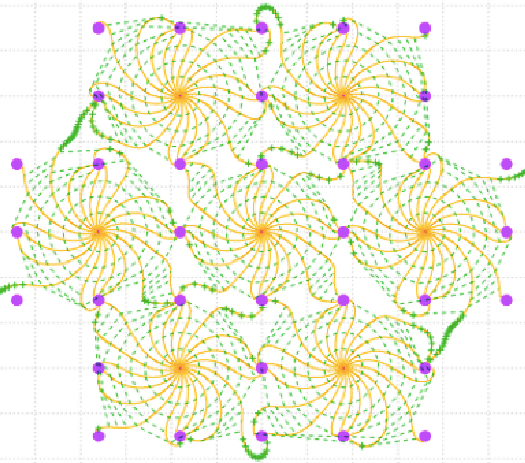
\includegraphics[width=0.5\linewidth]{figures/experimental_setup/electronsInCDC.pdf}
  \label{fig-sense-wires}
\end{SCfigure}


\begin{figure}
  \centering
  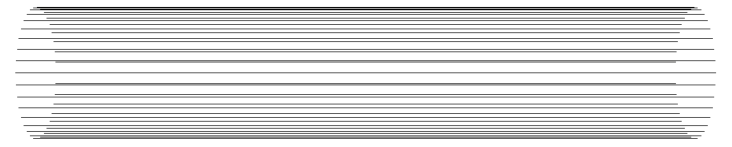
\includegraphics{figures/experimental_setup/axialLayers.pdf}
  
  \vspace*{1.5cm}
  
  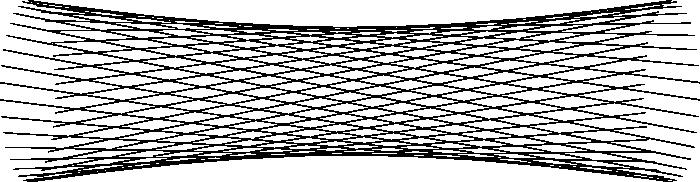
\includegraphics{figures/experimental_setup/stereoLayers.pdf}
  \caption{Drawing sketching the axial (top) and stereo wires in the CDC. The skewing against the beamline of the stereo (bottom) wires is exaggerated. Taken from \cite{oliver}.}
  \label{fig-axial-stereo}
\end{figure}

\begin{figure}
  \centering
  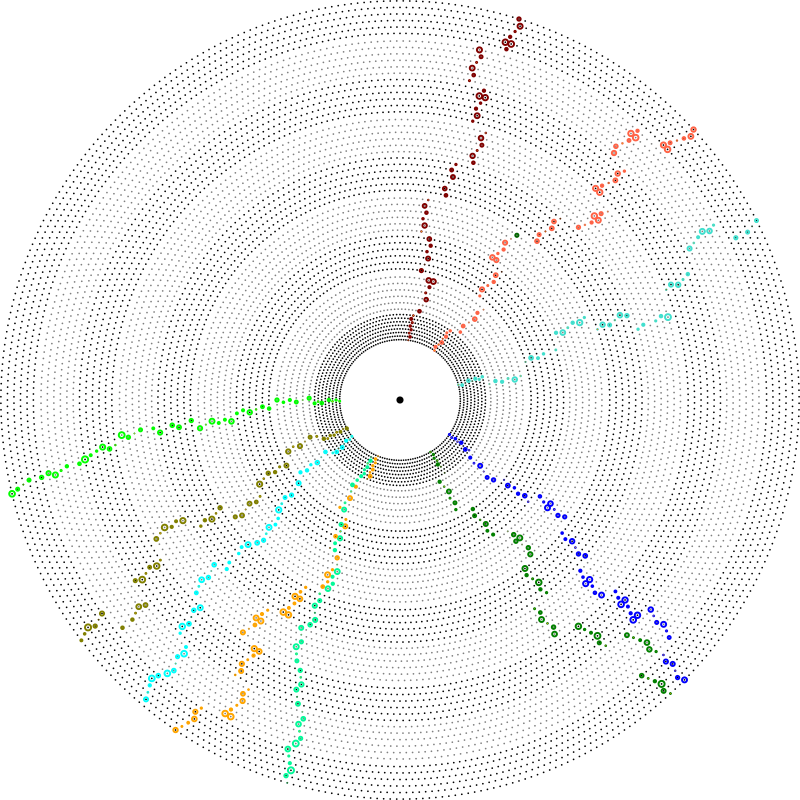
\includegraphics[width=0.8\linewidth]{figures/experimental_setup/eventDisplayPionGun.png}
  \caption{Simulated event of the passage of 10 $\Ppi^\pm$ with approximately $\unit[10]{GeV}$ through the CDC shown in a plane perpendicular to the beam axis. The interaction point is drawn as a black cirlce in the center. Each particle is colored differently to distinguish between them. Only the CDC detector is shown for better visuability. The wires are shown as gray (stereo) or black (axial) points. The hitten wires are depicted with their drift circles. The appearing disruption in the circular paths of the particle araise due to the stereo and axial wires.}
  \label{fig-axial-stereo}
\end{figure}



\subsection{VXD}
